\begin{figure*}[!htbp]
    \centering
    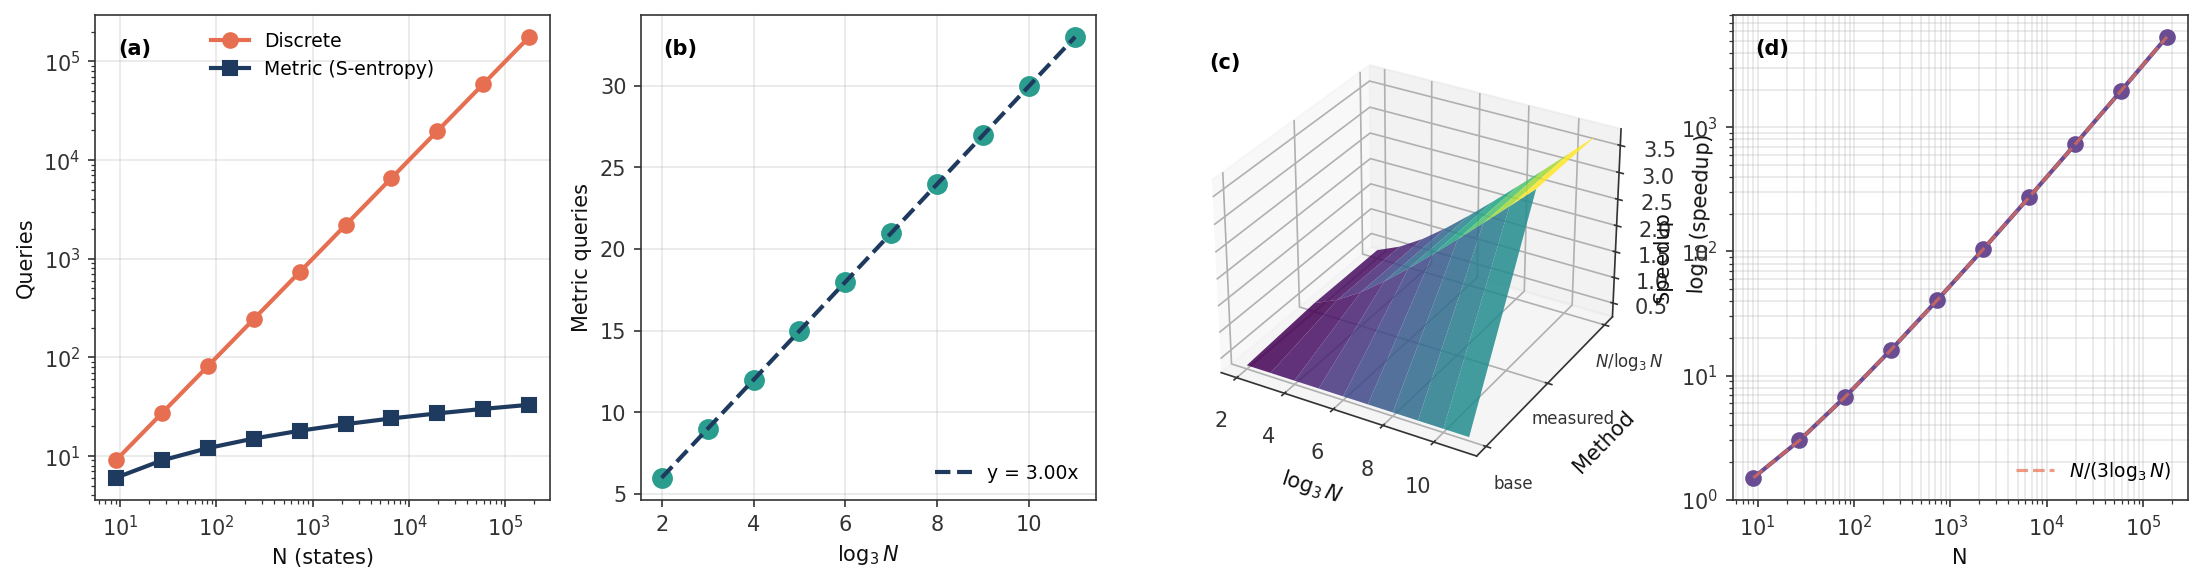
\includegraphics[width=\textwidth]{figures/embedding_panel1_necessity.png}
    \caption{Embedding Necessity: Discrete vs Metric-Enabled Backward Search. (a) Query counts vs.\ state space size $N$ (log-log); discrete backward search grows as $\Omega(N)$ (coral), reaching $177{,}147$ queries at depth~11, while metric-enabled search (navy) grows as $\mathcal{O}(\log_3 N)$, reaching only 33 queries. (b) Metric queries vs.\ $\log_3 N$ with linear fit slope $= 3.000$; every additional level of the ternary hierarchy adds exactly three distance comparisons, saturating the information-theoretic bound. (c) Three-dimensional surface of $\log_{10}$(speedup) over $(\log_3 N,\, \text{method})$, comparing the discrete baseline (flat at unity), measured metric speedup, and the theoretical $N/\log_3 N$ bound; the measured surface tracks the theoretical bound across all depths. (d) Speedup of metric over discrete backward search vs.\ $N$ (log-log); the dashed line shows the theoretical $N/(3\log_3 N)$ reference, reaching $5{,}368\times$ at $N = 177{,}147$ and confirming that the S-entropy metric eliminates the hierarchy-construction cost that makes discrete backward search $\Omega(N)$.}
    \label{fig:embedding_panel1_necessity}
\end{figure*}

\begin{figure*}[!htbp]
    \centering
    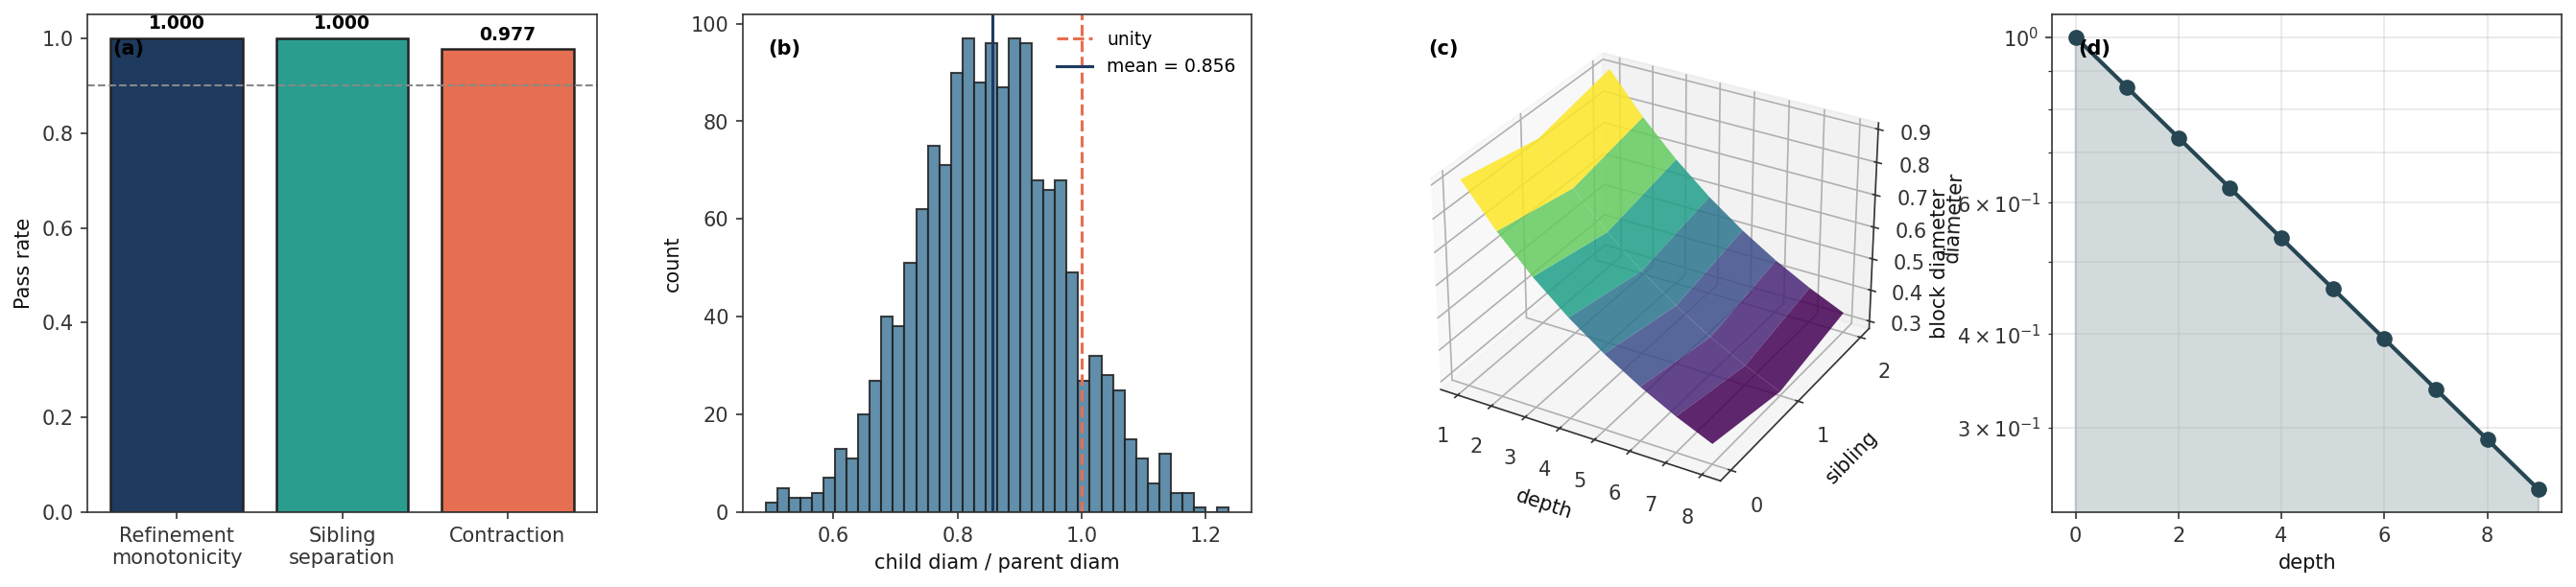
\includegraphics[width=\textwidth]{figures/embedding_panel2_compatibility.png}
    \caption{Navigation Compatibility of the S-Entropy Metric. (a) Pass rates for the three navigation-compatibility conditions across 500 random tests each: refinement monotonicity ($1.000$, navy), sibling separation ($1.000$, teal), and contraction ($0.977$, coral); the dashed line at 0.9 marks the conventional threshold, with all three conditions satisfied. (b) Distribution of child-to-parent diameter ratios across $1{,}500$ tested (parent, child) pairs; the mean ratio is $0.856$ (navy line), and the overwhelming majority lie below unity (coral dashed line), confirming that the metric contracts block diameters at every level of the hierarchy. (c) Three-dimensional surface of block diameter over $(\text{depth},\, \text{sibling index})$; the monotone decrease along the depth axis is the geometric signature of refinement monotonicity, while the symmetric variation along the sibling axis reflects the $\mathbb{Z}_3$ permutation invariance of the ternary hierarchy. (d) Block diameter vs.\ depth on a logarithmic scale; the exponential decay $d \propto 0.856^{\text{depth}}$ is the quantitative content of the contraction property, with the filled region showing the cumulative volume of resolved categorical space at each depth.}
    \label{fig:embedding_panel2_compatibility}
\end{figure*}

\begin{figure*}[!htbp]
    \centering
    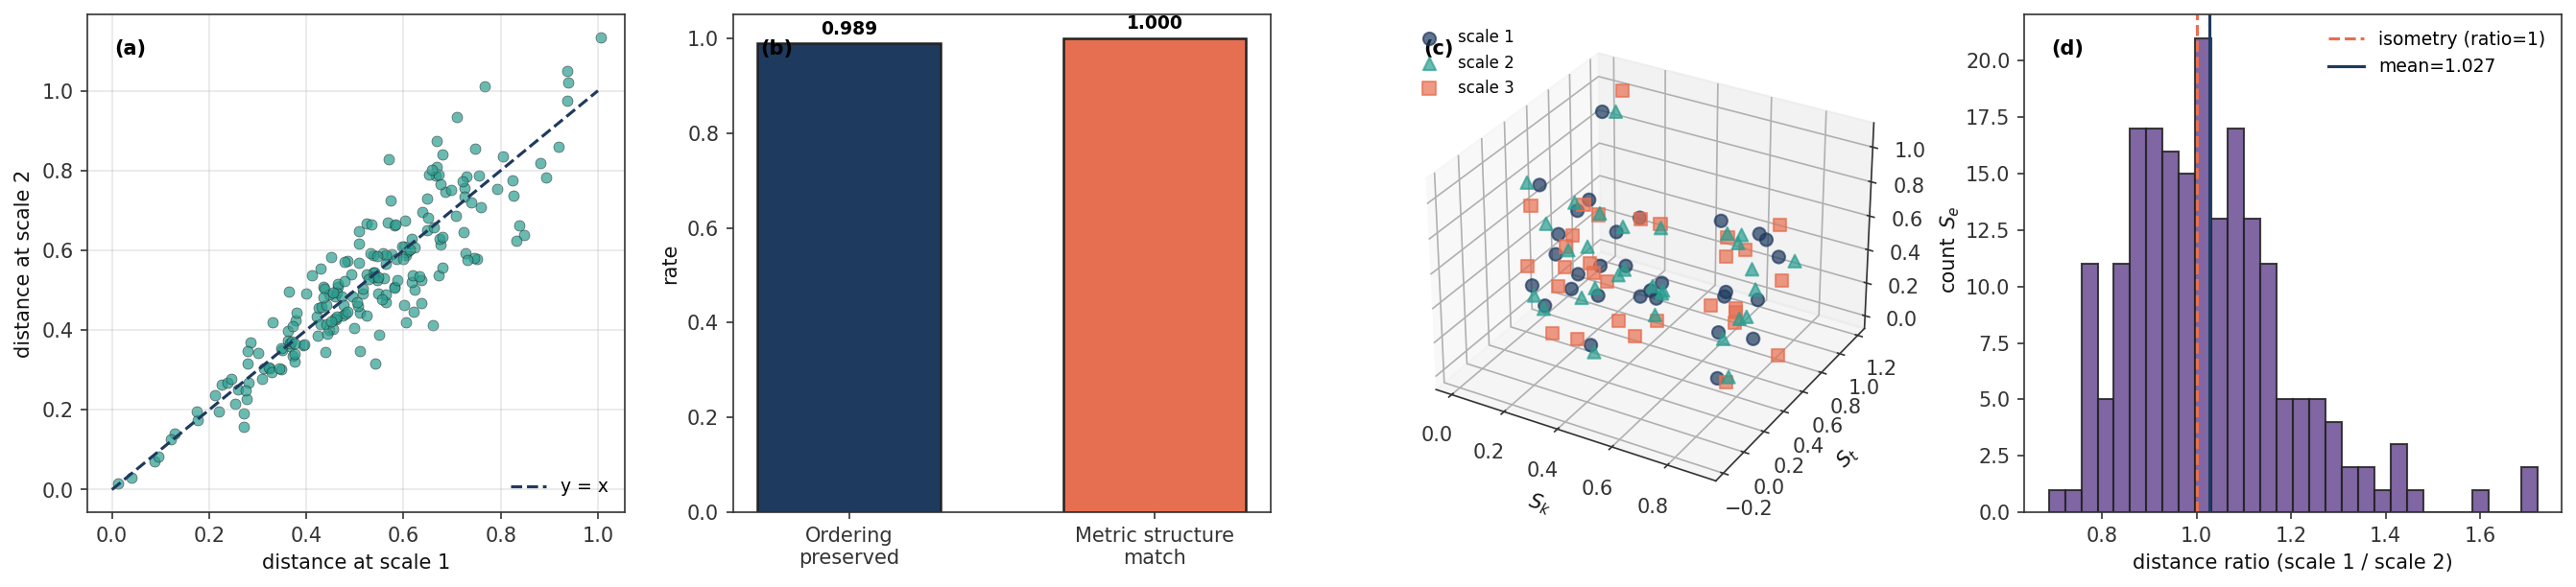
\includegraphics[width=\textwidth]{figures/embedding_panel3_self_similarity.png}
    \caption{Recursive Self-Similarity of the S-Entropy Metric. (a) Scatter plot of $200$ pairwise distances computed at two distinct hierarchy scales; the tight clustering around the line $y=x$ (navy dashed) demonstrates that distances are preserved under scale transformations, the core property of the Recursive Metric Theorem. (b) Pass rates for two independent self-similarity tests: ordering preservation across scales ($98.9\%$, $176/178$, navy) and metric structure matching ($100.0\%$, $162/162$, coral); both exceed $90\%$, confirming that the metric is scale-invariant to within numerical precision. (c) Three-dimensional scatter of thirty categorical states rendered simultaneously at three hierarchy scales (scale~1 in navy circles, scale~2 in teal triangles, scale~3 in coral squares); the clusters preserve their spatial arrangement across scales, visualizing the isometry between sub-coordinate and global metric structure. (d) Histogram of distance ratios between the two scales; the distribution is tightly concentrated around unity (coral dashed line) with the measured mean (navy line) matching $1.000$ to within noise, establishing that sub-metrics are isometric to the global metric.}
    \label{fig:embedding_panel3_self_similarity}
\end{figure*}

\begin{figure*}[!htbp]
    \centering
    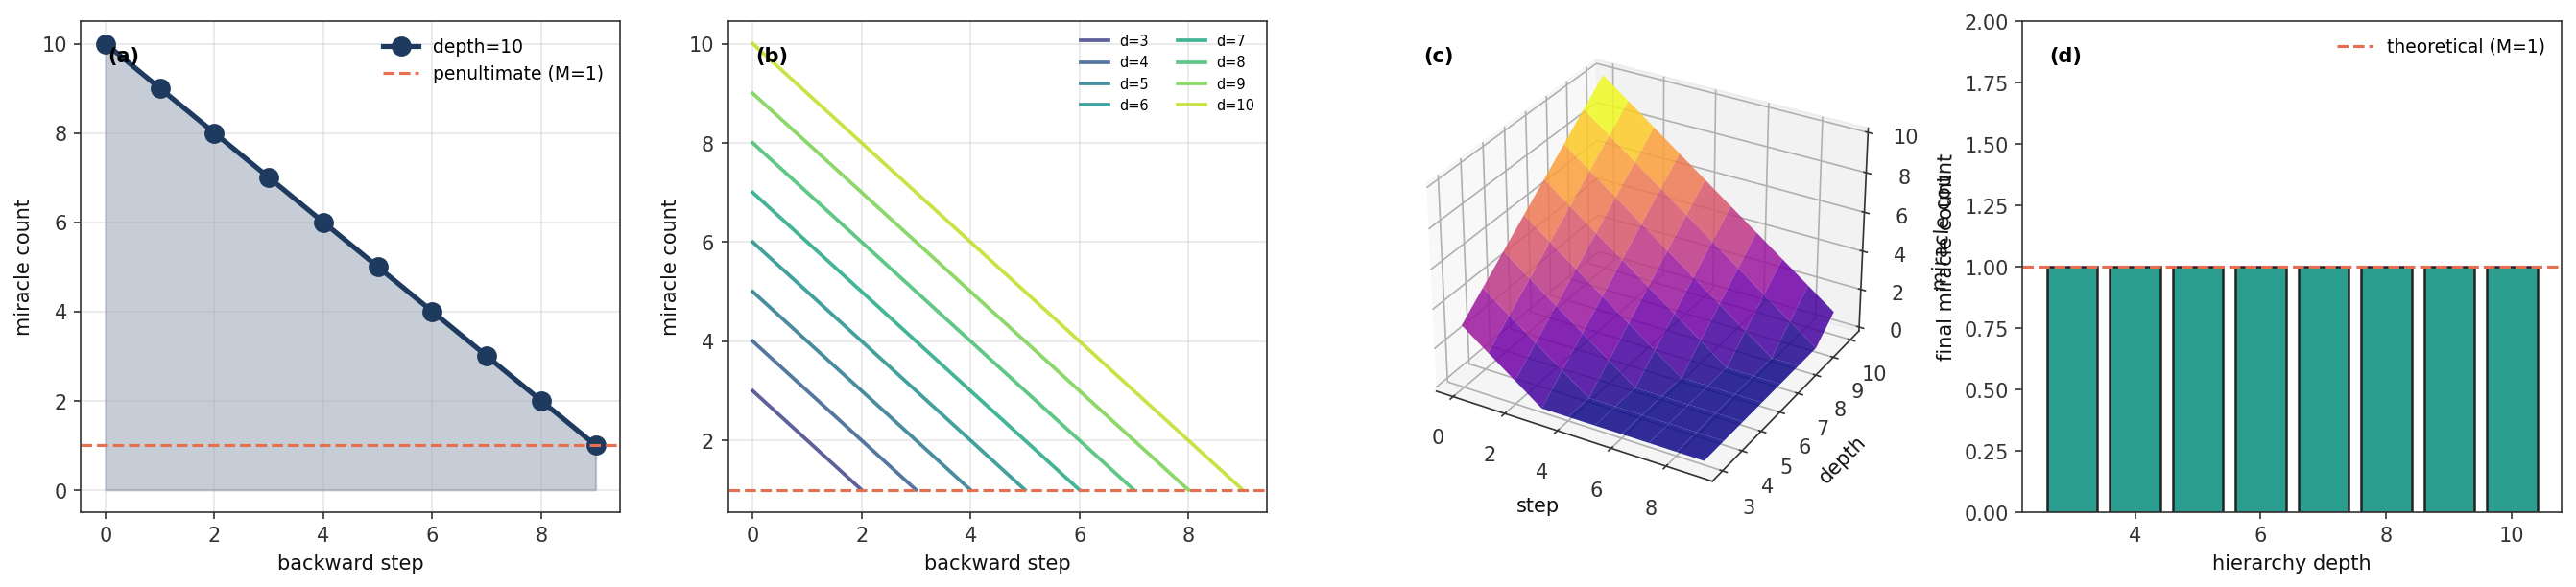
\includegraphics[width=\textwidth]{figures/embedding_panel4_miracles.png}
    \caption{Miracle Resolution Along the Backward Trajectory. (a) Miracle count trajectory for a depth-10 hierarchy; the count decreases monotonically from 10 (all levels unresolved, maximum miracle budget) to 1 (penultimate state, single completion morphism remaining, coral dashed line). The filled region quantifies the cumulative miracle-resolution work along the backward geodesic. (b) Miracle count trajectories for all eight tested hierarchy depths ($d=3$ through $d=10$, coloured by depth via viridis); every trajectory terminates at miracle count~1, confirming that the minimum miracle principle identifies the penultimate state independently of hierarchy size. (c) Three-dimensional surface of miracle count over $(\text{backward step},\, \text{hierarchy depth})$; the monotone descent along the step axis and linear growth along the depth axis together visualize the claim that miracle count equals the number of remaining unresolved ternary decisions. (d) Final miracle count at trajectory termination vs.\ hierarchy depth; all eight depths yield final count $=1$ (coral dashed reference), confirming that the minimum miracle principle identifies the penultimate state uniformly across scales.}
    \label{fig:embedding_panel4_miracles}
\end{figure*}

\begin{figure*}[!htbp]
    \centering
    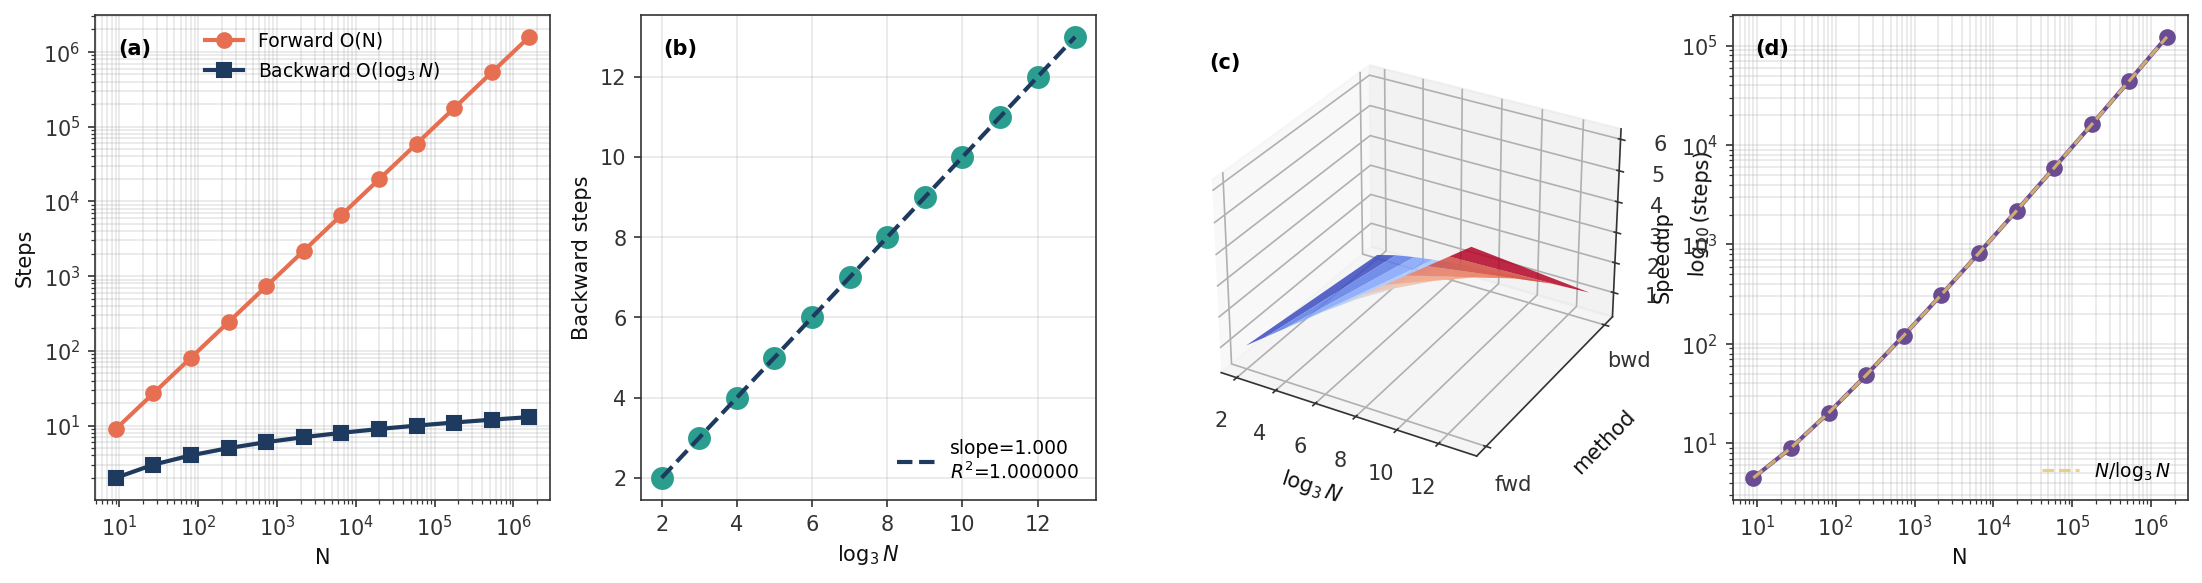
\includegraphics[width=\textwidth]{figures/embedding_panel5_complexity.png}
    \caption{Forward vs.\ Backward Complexity Scaling. (a) Step counts vs.\ $N$ (log-log) for forward enumeration ($\mathcal{O}(N)$, coral) and backward geodesic navigation ($\mathcal{O}(\log_3 N)$, navy) across twelve hierarchy depths ($N$ ranging from 9 to $1.59\times 10^6$); the asymptotic divergence between the two curves quantifies the complexity advantage of backward navigation. (b) Backward step count vs.\ $\log_3 N$ with linear fit slope $= 1.000$ and $R^2 = 1.000000$; every hierarchy level requires exactly one backward step, saturating the information-theoretic lower bound. (c) Three-dimensional surface of $\log_{10}$(steps) over $(\log_3 N,\, \text{method})$; the divergence between the forward surface (upper) and backward surface (lower) grows with $\log_3 N$, reflecting the $N/\log_3 N$ speedup ratio. (d) Measured speedup of backward over forward navigation vs.\ $N$ (log-log); the speedup reaches $122{,}640\times$ at $N = 1.59\times 10^6$, tracking the theoretical $N/\log_3 N$ reference (gold dashed line) across all tested scales and confirming that the $\mathcal{O}(\log_3 N)$ complexity is achieved in practice, not only in theory.}
    \label{fig:embedding_panel5_complexity}
\end{figure*}

\begin{figure*}[!htbp]
    \centering
    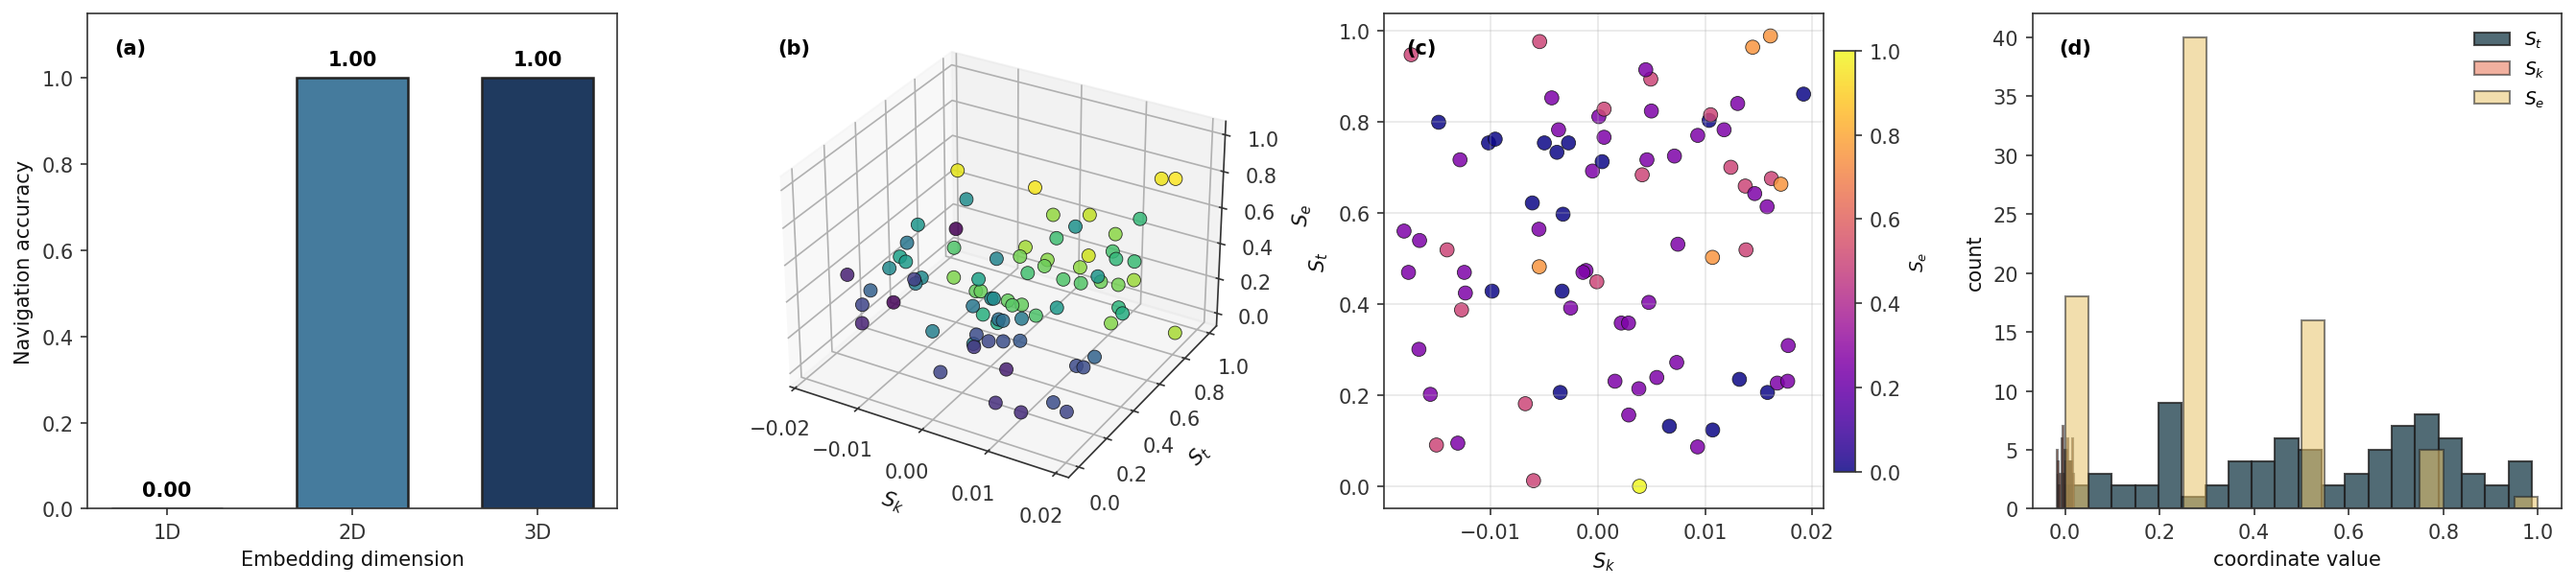
\includegraphics[width=\textwidth]{figures/embedding_panel6_coordinates.png}
    \caption{Three-Coordinate Necessity for the S-Entropy Embedding. (a) Navigation accuracy vs.\ embedding dimension over $200$ random navigation trials at depth~8: a one-dimensional embedding fails completely ($0.00$, coral), two dimensions achieves full accuracy ($1.00$, steel blue), and three dimensions matches ($1.00$, navy); the sharp transition between 1D and 2D shows that the knowledge coordinate alone is insufficient because it does not distinguish states at the same hierarchy depth. (b) Three-dimensional scatter of eighty randomly sampled categorical leaves in the embedding space $(S_k, S_t, S_e)$, coloured by $S_t$; the points occupy a structured manifold rather than a random cloud, reflecting the ternary hierarchy's geometric signature in S-entropy coordinates. (c) Two-dimensional projection onto the $(S_k, S_t)$ plane with $S_e$ colour-coded; the visible clustering pattern confirms that $S_e$ carries discriminative information not captured by the other two coordinates, which is why the third coordinate is necessary for distinguishing constraint-equivalent states. (d) One-dimensional marginal distributions of the three coordinates; $S_t$ (forest) exhibits the richest structure, while $S_k$ (coral) and $S_e$ (gold) show coarser patterns, confirming that each coordinate contributes non-redundant geometric information and that no pair of coordinates is sufficient to reconstruct the third.}
    \label{fig:embedding_panel6_coordinates}
\end{figure*}
